\newpage
\section{Vektorräume mit Skalarprudukt \texorpdfstring{$K=\mr$}{K=R}}
\subsection{Einführung}
	$\mr^2$

	\begin{tikzpicture}
		\draw (0,3) -- (0,0) -- (4,0);
		\draw [->] (0,0) -- (3.5,2.5);
		\draw (3.5,.1) -- (3.5,-.1) node[anchor = north]{$x_1$};
		\draw (.1,2.5) -- (-.1,2.5) node[anchor = east]{$x_2$};
		\draw [dotted] (3.5,0) -- (3.5,2.5) node[anchor = west]{$v\leftrightarrow\lrv{x_1\\x_2}$};
	\end{tikzpicture}

	\textbf{Länge} von $v$: $\lrabs{\lrabs{v}}=+\sqrt{x_1^2+x_2^2}$ (Pythagoras)

	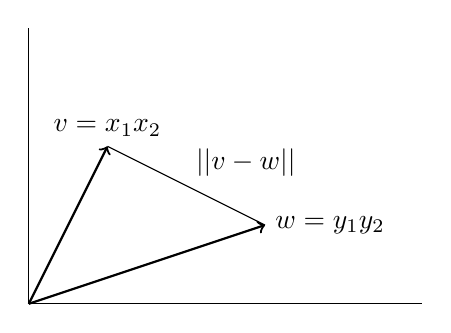
\begin{tikzpicture}
    \draw (0,0) -- (5,0);
    \draw (0,0) -- (0,3.5);
    \draw [->, thick] (0,0) -- (1,2) node [anchor=south] {$v=\lrv{x_1\\x_2}$};
    \draw [->, thick] (0,0) -- (3,1) node [anchor=west] {$w=\lrv{y_1\\y_2}$};
    \draw (3,1) -- node [anchor=south west] {$||v-w||$} (1,2);
  \end{tikzpicture}

	\textbf{Abstand} von $v,w$: $d\lrr{v,w}=\lrabs{\lrabs{v-w}}=+\sqrt{\lrr{x_1-y_1}^2+\lrr{x_2-y_2}^2}$

	\textbf{Winkel} (über Pythagoras)

  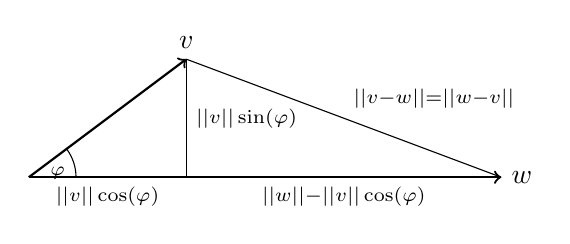
\begin{tikzpicture}
    \draw (2,0) -- node [anchor=west] {$\scriptstyle ||v||\sin(\varphi)$} (2,1.5);
    %\node [anchor=south] at (2,1.5) {$v$};
    %\node [anchor=west] at (6,0) {$w$};
    \path (2,0) -- node [anchor=north] {$\scriptstyle ||w||-||v||\cos(\varphi)$} (6,0);
    \path (0,0) -- node [anchor=north] {$\scriptstyle ||v||\cos(\varphi)$} (2,0);
    \draw [->, thick] (0,0) -- (2,1.5) node [anchor=south] (v) {$v$};
    \draw [->, thick] (0,0) -- (6,0) node [anchor=west] (w) {$w$};
    \draw (2,1.5) -- node [anchor=south west] {$\scriptstyle||v-w||=||w-v||$} (6,0);
    \draw (6mm,0mm) arc (0:36:6mm);
    \draw (.15,-.15) node [anchor=south west] {$\scriptstyle\varphi$};
  \end{tikzpicture}

	$\lrabs{\lrabs{v-w}}^2=\lrabs{\lrabs{v}}^2\sin^2\lrr{\varphi}+\lrr{\lrabs{\lrabs{w}}-\lrabs{\lrabs{w}}\cos\lrr{\varphi}}^2\\
	=\lrabs{\lrabs{v}}^2+\lrabs{\lrabs{w}}^2-2\lrabs{\lrabs{v}}\lrabs{\lrabs{w}}\cos\lrr{\varphi}$\\
	Mit Kosinussatz ($\sin^2(\varphi)+\cos^2(\varphi)=1$)

	$\lrabs{\lrabs{v-w}}^2=\lrr{x_1-y_1}^2+\lrr{x_2-y_2}^2=x_1^2+y_1^2+x_2^2+y_2^2-2x_1y_1-3x_2y_2$\\
	$\lrabs{\lrabs{v}}^2+\lrabs{\lrabs{w}}^2-2\lrr{x_1y_1+x_2y_2}$

	Es folgt:$\underbrace{x_1y_1+x_2y_2}_{\smt{Skalarprodukt}}=\lrabs{\lrabs{v}}\lrabs{\lrabs{w}}\cos\lrr{\varphi}$

\subsection{Definition: Standardskalarprodukt}
	Seien $v,w\in\mr^n$ mit $v=\lrv{x_1\\\vdots\\x_n}, w=\lrv{y_1\\\vdots\\y_n}$\\
	Das \textbf{(Standard-) Skalarprodukt} von $v$ und $w$ ist\\
	$\lrr{v\mid w}=x_1y_1+x_2y_2+\dots+x_ny_n\;\;\in\mr$\\
	(Skalarprodukt von zwei Vektoren ergibt ereele Zahl)

	Es gilt
	\subExBegin{(1)}
		\item $\lrr{v\mid v}\geq 0$, $\lrr{v\mid v}=0\Leftrightarrow v=\sigma$\\
			(positiv definit)
		\item $\lrr{v\mid w}=\lrr{w\mid v}$ (symmetrisch)
		\item $\lrr{v\mid aw}=a\lrr{v\mid w}$\\
			$\lrr{v\mid w_1+w_2}=\lrr{v\mid w_1}+\lrr{v\mid w_2}$\\
			$\forall v,w,w_1,w_2\in\mr^n$ und $\forall a\in\mr$\\
			(Linearität im 2.Argument)
	\subExEnd
	Mit (2) und (3) folgt
	\subExBegin{(1)}
		\item[(4)] $\lrr{av\mid w}=a\lrr{v\mid w}$\\
			$\lrr{v_1+v_2\mid w}=\lrr{v_1\mid w}+\lrr{v_2\mid w}$\\
			$\forall v,v_1,v_2,w\in V, a\in\mr$\\
			Es gilt dann auch:\\
			$\lrr{\sigma\mid v}=\lrr{v\mid\sigma}=0$
	\subExEnd
	Dann heißt $V$ \textbf{Euklidischer} Vektorraum oder \textbf{Skalarproduktraum}.

\subsection{Beispiele}
	\subExBegin{a)}
		\item Das Standardskalarprodukt auf $\mr^n$ ist das Skalarprodukt im Sinne von 8.2
		\item $V$ ist $n$-dimensionaler $\mr$-Vektorraum.\\
			$\lrr{v_1,\dots,v_n}$ Basis von $V$.\\
			$v=\limsum{i=1}{n}a_iv_i$, $w=\limsum{i=1}{n}b_iv_i$\\
			$\lrr{v\mid w}:=\limsum{i=1}{n}a_ib_i$\\
			Skalarprodukt auf $V$.\\
			Standardskalarprodukt auf $\mr^n$ ist Spezialfall:\\
			Wähle Basis $\lrr{e_1,\dots,e_n}$
		\item $a,b\in\mr, a<b$\\
			$C\lra{a,b}=$ Vektorraum der stetigen Funktionen $\lra{a,b}\rightarrow\mr$\\
			$f,g\in C\lra{a,b}$:\\
			$\lrr{f\mid g}:=\limint{a}{b}f(x)g(x)\intd{x}\in\mr$\\
			Skalarprodukt auf $C\lra{a,b}$.\\
			\subExBegin{(1)}
				\item $\lrr{f\mid f}=\limint{a}{b}f^2(x)\intd{x}\geq 0$\\
					$f\neq 0: \lrr{f\mid f}>0$\\
					Dann $f^2>0$, also $\lrr{f\mid f}> 0$\\
					($f$ stetig nach MAthe 2)
			\subExEnd
	\subExEnd

\subsection{Satz: Cauchy-Schwarz'sche Ungleichung}
	$V$ Euklidischer Vektorraum.\\
	Dann $\forall v,w\in V: \lrr{v\mid w}^2\leq\lrr{v\mid v}\cdot\lrr{w\mid w}$\\
	Gleichheit $\Leftrightarrow v,w$ lin. abhängig

	\textbf{Beweis}

	Ist $w=\sigma$, so stimmt die Aussage des Satzes. Ist $w\neq 0$, so setze $aO\frac{\lrr{v\mid w}}{\lrr{w\mid w}}\in\mr$\\
	(Da $\lrr{w\mid w}> 0 (1)$)

	$0\ouset{\leq}{}{(1)}\lrr{v-aw\mid v-aw}\ouset{=}{}{(3)}\lrr{v-aw\mid v}-a\lrr{v-aw\mid w}$\\
	$\ouset{=}{}{(4)}\lrr{v\mid v}-a\lrr{w\mid v}-a\lrr{v\mid w}+a^2\lrr{w\mid w}$\\
	$\ouset{=}{}{(2)}\lrr{v\mid v}-2a\lrr{v\mid w}+a^2\lrr{w\mid w}$\\
	$\ouset{=}{}{\smt{Def. a}}\lrr{v\mid v}-\frac{2\lrr{v\mid w}^2}{\lrr{w\mid w}}+\frac{\lrr{v\mid w}^2}{\lrr{w\mid w}}$\\
	$=\lrr{v\mid v}-\frac{\lrr{v\mid w}^2}{\lrr{w\mid w}}$\\
	$\ouset{\Rightarrow}{}{\lrr{w\mid w}>0} 0\leq\lrr{v\mid v}\lrr{w\mid w}-\lrr{v\mid w}^2$\\
	Gleichheit $\Leftrightarrow\lrr{v-aw\mid v-aw}=0\ouset{\Leftrightarrow}{}{(1)}v=aw$, $v,w$ linear unabhängig.

\subsection{Definition: Euklidsche Norm und Euklidscher Abstand}
	$V$ Euklidischer Vektorraum mit Skalarprodukt $\lrr{.\mid .}$
	\subExBegin{a)}
		\item Für $v\in V$ ist die \textbf{(Euklidische) Norm} von $v$ durch $\lrabs{\lrabs{v}}:=+\sqrt{\lrr{v\mid v}}$
		\item Für $v,w\in V$ ist der \textbf{Euklidscher Abstand} von $v$ und $w$ definiert durch\\
			$d\lrr{v,w}:=\lrabs{\lrabs{v-w}}$
	\subExEnd
	Damit lässt sich 8.4 schreiben als: $\lrabs{\lrr{v\mid w}}\leq\lrabs{\lrabs{v}}\cdot\lrabs{\lrabs{w}}$

\subsection{Beispiele}
	\subExBegin{a)}
		\item Standardskalarprodukt auf $\mr^n$:\\
			$v=\lrv{x_1\\\vdots\\x_n}, w=\lrv{y_1\\\vdots\\y_n}$\\
			$\lrabs{\lrabs{V}}=+\sqrt{x_1^2+\dots+x_n^2}$\\
			$d\lrr{v,w}=+\sqrt{\lrr{x_1-y_1}^2+\dots+\lrr{x_n-y_n}^2}$\\
			$n=2,3$ entspricht geometrischer Länge
		\item $V=C\lra{a,b}$\\
			$\lrr{f\mid g}=\limint{a}{b}f\lrr{x}g\lrr{x}\intd{x}, \lrabs{\lrabs{f}}+\sqrt{\limint{a}{b}f(x)^2\intd{x}}$
	\subExEnd

\subsection{Satz: Eigenschaften der Norm}
	$V$ Euklidscher Vektorraum mit Euklidscher Norm $\lrabs{\lrabs{.}}$\\
	Dann gilt $v,w\in V, a\in\mr$
	\subExBegin{(1)}
		\item $\lrabs{\lrabs{v}}\geq 0; \lrabs{\lrabs{v}}=0\Leftrightarrow v=\sigma$ (Definitheit)
		\item $\lrabs{\lrabs{av}}=\lrabs{a}\cdot\lrabs{\lrabs{v}}$ (absolute Homogenität)
		\item $\lrabs{\lrabs{v+w}}\leq\lrabs{\lrabs{v}}+\lrabs{\lrabs{w}}$ (Dreiecksungleichung)

			$\mr^2$
			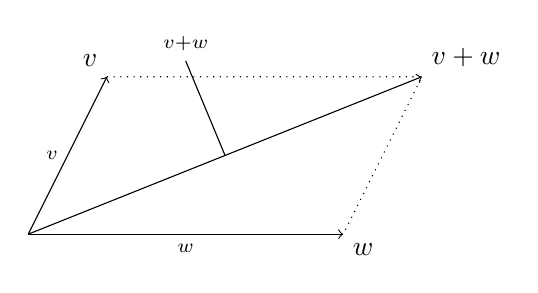
\begin{tikzpicture}
				\draw [->] (0,0) -- (2,0) node[anchor= north]{$\scriptstyle \lrabs{\lrabs{w}}$} -- (4,0) node[anchor= north west]{$w$};
				\draw [->] (0,0) -- (0.5,1) node[anchor= east]{$\scriptstyle \lrabs{\lrabs{v}}$} -- (1,2) node[anchor= south east]{$v$};
				\draw [->] (0,0) -- (5,2) node[anchor= south west]{$v+w$};
				\draw [dotted] (1,2) -- (5,2) -- (4,0);
				\draw (2.5,1) -- (2,2.2) node[anchor= south]{$\scriptstyle \lrabs{\lrabs{v+w}}$};
			\end{tikzpicture}
		\item $\lrabs{\lrabs{v+w}}^2=\lrabs{\lrabs{v}}^2+\lrabs{\lrabs{w}}^2+2\lrr{v\mid w}$
		\item $\lrabs{\lrabs{v+w}}^2+\lrabs{\lrabs{v-w}}^2=2\lrr{\lrabs{\lrabs{v}}^2+\lrabs{\lrabs{w}}^2}$ (Parallelogrammgleichung)

			$\mr^2$
			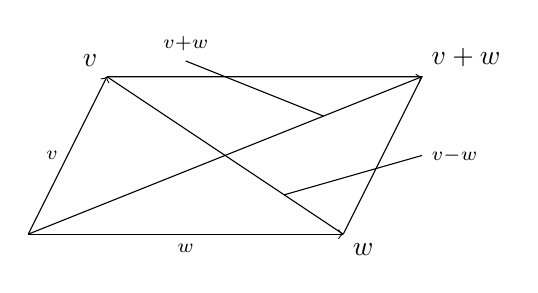
\begin{tikzpicture}
				\draw [->] (0,0) -- (2,0) node[anchor= north]{$\scriptstyle \lrabs{\lrabs{w}}$} -- (4,0) node[anchor= north west]{$w$};
				\draw [->] (0,0) -- (0.5,1) node[anchor= east]{$\scriptstyle \lrabs{\lrabs{v}}$} -- (1,2) node[anchor= south east]{$v$};
				\draw (1,2) -- (5,2) -- (4,0);
				\draw (3.75,1.5) -- (2,2.2) node[anchor= south]{$\scriptstyle \lrabs{\lrabs{v+w}}$};
				\draw [->] (0,0) -- (5,2) node[anchor= south west]{$v+w$};
				\draw (1,2) -- (4,0);
				\draw (3.25,0.5) -- (5,1) node[anchor=west]{$\scriptstyle \lrabs{\lrabs{v-w}}$};
			\end{tikzpicture}
	\subExEnd
	\textbf{Beweis}

		(1),(2) sind klar.
		(3),(4):\\
		$\lrabs{\lrabs{v+w}}^2=\lrabs{v+w\mid v+w}=\lrr{v\mid v}+\lrr{w\mid w}+2\lrr{v\mid w}\leftarrow (4)$\\
		$\ouset{\leq}{}{\smt{8.4}}\lrr{v\mid v}+\lrr{w\mid w}+2\sqrt{\lrr{v\mid v}\lrr{w\mid w}}$\\
		$=\lrr{\sqrt{\lrr{v\mid v}}+\sqrt{\lrr{w\mid w}}}^2=\lrr{\lrabs{\lrabs{v}}+\lrabs{\lrabs{w}}}^2$\\
		(5) folgt aus (4)

\subsection{Bemerkung}
	Für $\mr$-Vektorräume nennt man jede Funktion $\lrabs{\lrabs{.}}:V\rightarrow\mr_{\geq 0}$ mit Eigenschaften (1),(2),(3) aus 8.7 eine \textbf{Norm}.\\
	Dann gibt es auch andere Normen als solche, die über Skalarprodukte definiert werden.\\
	Zum Beispiel $\mr^n, \lrabs{\lrabs{\lrv{x_1\\\vdots\\x_n}}}_{\smt{max}}:=\mbox{max}\lrc{\lrabs{x_i}:i=1,\dots,n}$

\subsection{Definition: Winkel, orthogonal und Orthogonalraum}
	\subExBegin{a)}
		\item C-S-Ungleichung 8.4. mit $v\neq\sigma, w\neq\sigma$:\\
			$\frac{\lrabs{\lrr{v\mid w}}}{\lrabs{\lrabs{v}}\lrabs{\lrabs{w}}}\leq 1$\\
			Das heist $-1\leq\frac{\lrr{v\mid w}}{\lrabs{\lrabs{v}}\lrabs{\lrabs{w}}}\leq 1$\\
			Daher gibt es geunau ein $\varphi\in\lra{0,\pi}$ mit $\frac{\lrr{v\mid w}}{\lrabs{\lrabs{v}}\lrabs{\lrabs{w}}}=\cos\lrr{\varphi}$\\
			($\mr^2$: Standarskalarprodukt: $\varphi=$ Winkel zwischen $v,2$)\\
			$\varphi$ heißt der \textbf{Winkel} zwischen $v$ und $w$ $\lrr{0\leq\varphi\leq\pi}$
		\item $v,w$ heißen \textbf{orthogonal} (senkrecht), falls $\lrr{v\mid w}=0$\\
			(das heißt Winkel zwischen $v$ und $w$ ist $\frac{\pi}{2}(\hat{=}90^\circ$\\
			$\sigma$ ist orthogonal zu allen Vektoren. $v \perp w$
		\item $M\mpo V$, so $M^\perp=\lrc{w\in V:\lrr{v\mid w}=0\forall v\in M}$\\
			\textbf{Orthogonalraum} zu $M$.

			\textbf{Beispiel} $\mr^2$ Standardskalarprodukt.\\
				$M=\lrc{\lrv{1\\2}}$\\
				$\lrr{\lrv{x\\y}\mid\lrv{1\\2}}=0$\\
				$x+2y=0\Leftrightarrow x=-2y$\\
				$\Rightarrow M^\perp=\lrc{\lrv{-2y\\y}: y\in\mr}=\lrg{\lrv{2\\-1}}_\mr$
	\subExEnd

\subsection{Bemerkung}
	Sind $v,w$ orthogonal, so $\lrabs{\lrabs{v+w}}^2=\lrabs{\lrabs{v}}^2+\lrabs{\lrabs{w}}^2$ (Satz von Pythagoras)

\subsection{Beispiele}
    \begin{enumerate}[a)]
	\item $\mr^n$, Standardskalarprodukt $e_1,\dots,e_n$ kanonische Basis.\\
		$\lrabs{\lrabs{e_i}}=1\qquad\lrr{e_i\mid e_j}=0$ für $i\neq j$
	\item $\mr^3$, Standardskalarprodukt\\
		$v=\lrv{-1\\2\\1}, w=\lrv{2\\2\\4}$\\
		$\lrabs{\lrabs{v}}=\sqrt{6},\lrabs{\lrabs{w}}=\sqrt{24}$\\
		$\lrr{v\mid w}=-2+4+4=6$\\
		$\cos\lrr{\varphi}=\frac{6}{\sqrt{6}\sqrt{24}}=\frac{\sqrt{6}}{\sqrt{24}}=\sqrt{\frac{6}{24}}=\sqrt{\frac{1}{4}}=\frac{1}{2}$\\
		$\varphi=\frac{\pi}{3}\lrr{\hat{=}60^\circ}$
	%TODO Yannick%\item
%	$ v=\lrc{x_1\\x_2}\in\mr^2,\ v\neq\sigma $\\
%	$ \lrc{v}^\perp=\lrc{r\cdot\lrr{x_2\\x-_1}: x\ni\mr}=\lrg{\lrr{x_2\\-x_1}} $ (nachrechnen)\\
    \end{enumerate}
\subsection{Definition: Orthonormalsystem \& Orthonormalbasis}
	$ V $ Euklidischer Vektorraum, $ M\mpo V $
	\begin{enumerate}[a)]
		\item $ M $ heißt \textbf{Orthonormalsystem}, falls $ ||v||=1 $ für alle $ v\in M $ und falls $ (v|w)=0 $ für alle $ v,w\in M $, $ v\neq w $.
		\item Ist $ V $ endlicher dimensional, so heißt $ M $ \textbf{Orthonormalbasis} (ONB), dalls $ M $ sowohl Orthonormalsystem als auch Basis von $ V $ ist.
      \textbf{Beachte}: Ist $ (v_1,...,v_n) $ ONB von $ V $, $ v=\limsum{i=1}{n}c_iv_i $, so ist $ ||v||=\sqrt{\limsum{i=1}{n}c_i^2} $\\
      $ ((v|v)=\limsum{i=1}{n}c_iv_i\bigg|\limsum{c_jv_j}{})=\limsum{i,j}{}c_ic_j(v_i|v_j)=\limsum{i=1}{n}c_i^2 $
	\end{enumerate}
\subsection{Satz}
	\begin{enumerate}
		\item Ein Orthonormalsystem ist linear unabhängig.
		\item Ist $ M=\lrc{v_1,...,v_m} $, $ v\in V $, so ist $ v-\limsum{i=1}{m}(v|v_i)v_i\in M^\perp $.
	\end{enumerate}

	\textbf{Beweis:}
	\begin{enumerate}
		\item Zeige: Jede endliche Teilmenge von $ M $ ist linear unabhängig\\
			$ v_1,...,v_l\in M $. Seien $ c_i\in\mr $ mit $ \limsum{i=1}{l}c_iv_i=\sigma $.\\
			$ 0=(v_j|\sigma)=(v_i|\limsum{i=1}{l}c_iv_i)=\limsum{i=1}{l}c_i(v_j|v_i)=c_j $ für alle $ j=1 $, $ l $
		\item Sei $ v_j\in M $. $ (v_j|v-\limsum{i=1}{m}(v|v_i)v_i)=(v_j|v)-(v_j|\limsum{i=1}{m}(v|v_i))=(v_j|v)-\limsum{i=1}{m}(v|v_i)\underbrace{(v_j|v_i)}_{=0, i\neq j \quad =1, i=j}=(v_j|v)-(v|v_j)\cdot 1=0 $
	\end{enumerate}
\subsection{Das Gram- Schmidt'sche Orthonormalisierungsverfahren}
	Sei $ M=\lrc{W_1,...,W_m} $ linear unabhängige Menge von Vektoren in einem Euklidischen Vektorraum. Dann gibt es ein Orthogonalsystem $ \lrc{v_1,...,v_m} $ mit\\
	$ \lrg{v_1}=\lrg{w_1} $\\
	$ \lrg{v_1,v_2}=\lrg{w_1,w_2} $\\
	...\\
	$ \lrg{v_1,...,v_m}=\lrg{w_1,...,w_m} $, d.h.\\
	$ \lrg{v_1,...,v_i}=\lrg{w_1,...,w_i}\forall i\in\lrv{1,...,m} $\\
	Insbesondere: Jeder endlich dimensionaler Euklidischer VR besitzt ONB.\\
	\textbf{Beweis:}\\
	$ W_1=\sigma $. Setze $ v_1=\frac{1}{||w_1||}w_1 $\\
	$ ||v_1||=\lrabs{\lrabs{\frac{1}{||w_1||w_1}}}=\lrabs{\frac{1}{||w_1||}}||w_1||=1 $\\
	$ \lrg{v_1}=\lrg{w_1} $\\
	Sei schon Orthonormalsystem $ \lrv{v_1,...,v_i},\ i<m $ bestimmt mit $ \lrg{v_1,...,v_j}=\lrg{w_1,...,w_j},j=1,...,j $\\
	Konstruktion von $ v_{i+1} $.\\
	Setze $ v'_{i+1}=w_i+1-\limsum{j=1}{i}(v_j|w_{i+1})v_j $\\
	Sach 8.13b): $ (v_{i+1}|v_j)=0,\ j=1,...,i $.\\
	Da $ w_{i+1}\notin\lrg{w_1,...,w_i}=\lrg{v_1,...,v_i} $\\
	ist $ v'_{i+1}\neq\sigma $, setze $ v_{i+1}=\frac{1}{||v_{i+1}||}v'_{j+1} $. Dann gilt $ ||v_{i+1}||=1 $, $ (v_{i+1}|v_j)=0 $ für $ j=1,...,i $\\
	$ \lrg{v_1,...,v_i,v_{i+1}}=\lrg{v_1,...,v_i,v'_{i+1}}=\lrg{v_1,...,v_i,w_{i+1}}=\lrg{w_1,...,w_i,w_{i+1}} $

\subsection{Beispiel}
	\begin{enumerate}
		\item $ e_1,...,e_n $ ist ONB des $ \mr^n $ bezüglich Standardskalarprodukts.
		\item $ V=\mr^3 $, Standard- Skalarprodukt\\
			$ w_1=\lrv{1\\1\\1}, w_2=\lrv{1\\\\1},w_3=\lrv{1\\0\\0} $ linear unabhängig.\\
			Behauptung: ONB $ v_1,v_2,v_3 $ von $ \mr^3 $ von $ \mr^3 $ mit $ \lrg{v_1}=\lrv{w_1} $, $ \lrg{v_1,v_2}=\lrg{w_1,w_2} $\\
			$ \lrg{v_1,v_2,v_3}=\lrg{w_1,w_2,w_3}=\mr^3 $\\
			8.14: $ v_1=\frac{1}{\sqrt{3}}w_1=\frac{1}{\sqrt{3}}\lrv{1\\1\\1} $\\
			$ v_2'=w_2=(v_1|w_2)v_1=\lrv{1\\1\\2}-\frac{1}{3}\cdot 4\cdot\lrv{1\\1\\1}=\lrv{-1/3\\-1/3\\2/3}\\
			||v_2'||=\frac{\sqrt{6}}{3} $\\
			$ v_2=\frac{1}{||v_j||}\cdot v_2'=\frac{1}{\sqrt{6}}\lrv{-1\\-1\\2} $\\
			$ v_3'=\lrv{1\\0\\0}-\frac{1}{3}\lrr{\lrv{1\\1\\1}|\lrv{1\\0\\0}}\cdot\lrv{1\\1\\1}-\frac{1}{6}\lrr{\lrv{-1\\-1\\2}|\lrv{1\\0\\0}}\lrv{-1\\-1\\2}\\
			=\lrv{1\\0\\0}-\frac{1}{3}\lrv{1\\1\\1}+\frac{1}{6}\lrv{-1\\-1\\2}=\lrv{1/2\\-1/2\\0},\ ||v_3'||=\frac{\sqrt{2}}{2} $\\
			$ v_3=\frac{1}{\sqrt{2}}\lrv{1\\-1\\0} $
	\end{enumerate}

\subsection{Satz}
    $ V $ endlich dimensionaler Euklidischer Vektorraum.\\
    $ U $ Unterraum von $ V $.
    \begin{enumerate}[a)]
        \item $ V=U\oplus U^\perp $\\
        (d.h. $ V=U+U^\perp,U\mand U^\perp=\lrc{\mvoid} $)\\
        Insbesondere $ \dim(V)=\dim(U)+\dim(U^\perp) $
        \item $ \lrr{U^\perp}^\perp=U $
    \end{enumerate}

    \textbf{Beweis:}
    \begin{enumerate}[a)]
        \item $ w_1,...,w_m $ Basis von $ U $.\\
        Ergänze zu Basis $ w_1,...,w_m,w_{m+1},...,w_n $ von $ V $.\\
        Wende Gram- Schmidt (8.14) auf $ w_1,...,w_n $ an.\\
        Liefert ONB $ v_1,...,v_n $ von $ V $, $ \lrg{v_1,...,v_m}=\lrg{w_1,...,w_m}=U $\\
        $ v_{m+1},...,v_n $ orthogonal zu $ U $.\\
        $ \lrg{v_{m+1},...,v_n}\mpo U^\perp $\\
        $ V=\lrg{v_1,...,v_m}+\lrg{v_{m+1},...,v_n}\mpo U+U^\perp $\\
        $ V=U+U^\perp $\\
        $ v\in U\mand U^\perp\Rightarrow(v|v)=0 $
        $ \Rightarrow v=\sigma $\\
        $ U\mand U^\perp=\lrc{\sigma} $.
        \item $ U\mpo(U^\perp)^\perp $ klar.\\
        $ \dim\lrr{\lrr{U^\perp}^\perp}\ouset{=}{}{a)}\dim(V)-\dim(U^\perp)=U $
    \end{enumerate}

\subsection{Definition: Vektorprodukt}
	$ v=\lrv{x_1\\x_2\\x_3} $, $ w=\lrv{y_1\\y_2\\y_3}\in\mr^3 $\\
	$ v\times w=\lrr{x_2y_3-x_3y_2\\x_1y_1-x_1y_3\\x_1y_2-x_2y_1}\in\mr^3 $
	\textbf{Vektorprodukt} (Kreuzprodukt) von $ v $ und $ w $.

\subsection{Satz: Rechenregeln Kreuzprodukt}
	\begin{enumerate}
		\item $ (v\times w|v)=(v\times w|w)=0 $, d.h. steht senkrecht auf $ v $ und $ w $.
		\item  $ v\times w =-w\times v$
		\item  $ U\times(v+w)=(u\times v)+(u\times w)$\\
		$ u\times(av)=a(u\times v) $ für alle $ u,v,w\in V $, $ a\in\mr $ analog in der 1. Komponente
		\item  $ v\times w=\sigma\Leftrightarrow v,w $ sind linear abhängig.
		\item  $ v,w\neq\sigma $.\\
		$ \varphi\in\lra{0m\pi} $ Winkel zwischen $ v $ und $ w $, so $ ||v\times w||=||v||\cdot ||w||\cdot\sin(\varphi) $\\
		$ = $ Flächeninhalt des von $ v $ und $ w $ aufgespannten Parallelogramms.

		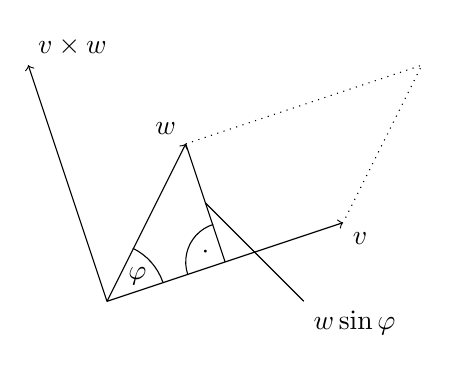
\begin{tikzpicture}
			\draw [->] (0,0) -- (3,1) node[anchor = north west]{$v$};
			\draw [->] (0,0) -- (1,2) node[anchor = south east]{$w$};
			\draw [dotted] (1,2) -- (4,3) -- (3,1);
			\draw (1,2) -- (1.5,0.5);
			\draw (1.25,1.25) -- (2.5,0) node[anchor = north west]{$\lrabs{\lrabs{w}}\sin\lrr{\varphi}$};
			\draw [->] (0,0) -- (-1,3) node[anchor = south west]{$v\times w$};
			\draw (19:0.75cm) arc (19:64:0.75cm);
			\draw (39.5:0.5cm) node{$\varphi$};

			\begin{scope}[shift={(1.5,0.5)}]
				\draw (107.5:0.5cm) arc (107.5:199:0.5cm);
				\draw (153.25:0.28cm) node{$\cdot$};
			\end{scope}
		\end{tikzpicture}
	\end{enumerate}
	\textbf{Beweis:}
	\begin{enumerate}
		\item Nachrechnen
		\item Nachrechnen
		\item Nachrechnen
		\item Nachrechnen
		\item $ ||v\times w||^2=(x_2y_3-x_3y_2)^2+(x_3y_1-x_1y_3)^2+(x_1y_2-x_2y_1)^2 $\\
		$ =(x_1^2+x_2^2+x_3^2)(y_1^2+y_2^2+y_3^2)-(x_1y_1+x_2y_2+x_3y_3)^2 $\\
		$ = ||v||^2 ||w||^2-(v|w)^2=||v||^2||w||^2-||v||^2||w||^2\cdot\cos(\varphi) $\\
		$ = ||v||^2||w||^2\sin^2(\varphi)$
		\item Folgt aus e)
	\end{enumerate}

\subsection{Bemerkung: Rechtssystem}
	$ v,w,v\times w $ bilden ein \textbf{Rechtssystem} (Drei- Finger- Regel):\\
	Faust, Daumen ausstrecken, Fingerspitzen von $ v $ nach $ w $ entlang des kleineren Winkels: Daumen zeigt in Richtung $ v\times w $.

\subsection{Beispiel}
	$ v=\lrv{1\\2\\0},w=\lrv{1\\1\\1} $\\
	Bestimme $ \lrg{v,w}^\perp $\\
	$ \dim\lrg{v,w}=2 $\\
	8.16: $ \dim\lrg{v,w}^\perp $\\
	$ \dim\lrg{v,w}^\perp=1 $\\
	$ \varepsilon\times w=\lrv{2\\-1\\-1} $\\
	$ \lrg{v,w}^\perp=\lrg{\lrv{2\\-1\\-1}} $
